\documentclass[11pt,a4paper]{article}

\usepackage[margin=1in]{geometry}
\usepackage{graphicx}
\usepackage{booktabs}
\usepackage{array}
\usepackage{longtable}
\usepackage{caption}
\usepackage{subcaption}
\usepackage{xcolor}
\usepackage{listings}
\usepackage{amsmath}
\usepackage{enumitem}
\usepackage{fancyhdr}
\usepackage{titlesec}
\usepackage[hidelinks]{hyperref}

\definecolor{codebg}{RGB}{245,245,245}
\definecolor{codekw}{RGB}{0,80,150}
\definecolor{codecomment}{RGB}{110,110,110}
\definecolor{codestring}{RGB}{140,20,20}

\lstset{
  backgroundcolor=\color{codebg},
  basicstyle=\ttfamily\small,
  keywordstyle=\color{codekw}\bfseries,
  commentstyle=\color{codecomment}\itshape,
  stringstyle=\color{codestring},
  showstringspaces=false,
  breaklines=true,
  frame=single,
  rulecolor=\color{gray!40},
  numbers=left,
  numberstyle=\tiny\color{gray},
  xleftmargin=1.8em,
  language=Python
}

\titleformat{\section}{\normalfont\Large\bfseries}{\thesection}{1em}{}
\titleformat{\subsection}{\normalfont\large\bfseries}{\thesubsection}{1em}{}

\pagestyle{fancy}
\fancyhf{}
\fancyhead[L]{ICS1512 -- Machine Learning Algorithms Laboratory}
\fancyhead[R]{Experiment 3}
\fancyfoot[C]{\thepage}
\renewcommand{\headrulewidth}{0.4pt}

\title{}
\date{}

\begin{document}

% ---------------- Title Page ----------------
\begin{titlepage}
\centering
\vspace*{1cm}
{\Large\bfseries Sri Sivasubramaniya Nadar College of Engineering, Chennai\par}
\vspace{0.2cm}
{\normalsize (An Autonomous Institution Affiliated to Anna University)\par}
\vspace{1.2cm}

{\Large\bfseries Machine Learning Algorithms Laboratory\par}
\vspace{0.3cm}
{\large ICS1512\par}
\vspace{1.5cm}

\begin{tabular}{|p{5.5cm}|p{7cm}|}
\hline
Degree \& Branch & M.Tech Computer Science \& Engineering \\
\hline
Semester & VI \\
\hline
Academic Year & 2026--2027 (Odd) \\
\hline
Batch & 2024--2029 \\
\hline
\end{tabular}

\vspace{1.8cm}
{\Large\bfseries Experiment 3\par}
\vspace{0.3cm}
{\large Regression Analysis using Linear and Regularized Models\footnote{\textbf{GitHub Repository: }\url{https://github.com/VijayaraaghavanKS/ML}}\par}
\vspace{2.5cm}

\begin{tabular}{ll}
Submitted by: & \textbf{Vijayaraaghavan K S} \\[4pt]
Register Number: & \textbf{3122247001066} \\[4pt]
Year: & III Year \\[4pt]
Programme: & M.Tech Integrated, CSE \\[4pt]
Faculty: & Dr. Poreddy Ajay Kumar Reddy \\[4pt]
\end{tabular}

\vfill
\end{titlepage}

\tableofcontents
\newpage

% ==========================================================
\section{Aim and Objective}
To implement Linear Regression alongside three regularized variants -- Ridge, Lasso, and Elastic Net -- for predicting a continuous target (the sanctioned loan amount), tune each model's regularization strength with cross-validated grid search, and use the results to reason about overfitting, underfitting, and the bias--variance trade-off rather than just reporting accuracy numbers.

% ==========================================================
\section{Problem Statement}
The input is a set of applicant details -- income, co-applicant income, credit score, age, requested loan term, number of dependents, property area, and existing-loan status -- and the output is a single continuous value, the sanctioned loan amount. The objective is to determine whether regularization (Ridge, Lasso, Elastic Net) meaningfully improves on plain Linear Regression for this specific dataset, and to use the coefficient behavior under each penalty to understand which applicant attributes actually drive the sanctioned amount.

% ==========================================================
\section{Theory}
Linear Regression fits $\hat y = Xw$ by minimizing ordinary least squares, $\mathcal{L}_{OLS}(w) = \tfrac{1}{2n}\sum_i (y_i - \hat y_i)^2$. It is unbiased when the linear assumption roughly holds, but with correlated or noisy features its coefficients can swing wildly between similar training samples -- that instability is exactly what regularization is meant to fix.

\begin{itemize}[nosep]
  \item \textbf{Ridge ($L_2$)} adds $\lambda \lVert w \rVert_2^2$ to the loss, shrinking all coefficients toward zero without ever setting them exactly to zero.
  \item \textbf{Lasso ($L_1$)} adds $\lambda \lVert w \rVert_1$, which can drive coefficients to exactly zero -- effectively doing feature selection as a side effect of fitting the model.
  \item \textbf{Elastic Net} blends both penalties ($\alpha$ controls overall strength, \texttt{l1\_ratio} controls the $L_1$/$L_2$ mix), aiming to get Lasso's sparsity without Lasso's instability when features are highly correlated.
\end{itemize}

% ==========================================================
\section{Machine Learning Algorithm}

\subsection{Linear Regression}
\textbf{Working principle:} fit a hyperplane through the training data that minimizes the sum of squared vertical distances between the observed and predicted target values.
\textbf{Mathematical formulation:} closed-form solution $\hat w = (X^TX)^{-1}X^Ty$ (the normal equation), or an iterative solver for large feature sets.
\textbf{Advantages:} fast to fit, fully interpretable coefficients, no hyperparameters to tune.
\textbf{Limitations:} sensitive to multicollinearity (unstable coefficients when features are correlated), assumes a linear relationship, and has no built-in mechanism to prevent overfitting on noisy or high-dimensional data.

\subsection{Ridge Regression}
\textbf{Working principle:} same least-squares objective as Linear Regression, plus an $L_2$ penalty that discourages large coefficient magnitudes.
\textbf{Mathematical formulation:} $\hat w = \arg\min_w \lVert y - Xw \rVert_2^2 + \lambda \lVert w \rVert_2^2$, solvable in closed form as $\hat w = (X^TX + \lambda I)^{-1}X^Ty$.
\textbf{Advantages:} stabilizes coefficients under multicollinearity, always has a unique closed-form solution (the $\lambda I$ term makes $X^TX+\lambda I$ invertible even when $X^TX$ is not).
\textbf{Limitations:} shrinks but never eliminates coefficients, so it does not perform feature selection; the right $\lambda$ has to be found by cross-validation.

\subsection{Lasso Regression}
\textbf{Working principle:} same objective as Ridge but with an $L_1$ penalty, which has the geometric property of driving some coefficients to exactly zero.
\textbf{Mathematical formulation:} $\hat w = \arg\min_w \lVert y - Xw \rVert_2^2 + \lambda \lVert w \rVert_1$, solved iteratively (coordinate descent) since there is no closed form.
\textbf{Advantages:} produces sparse, more interpretable models by zeroing out redundant features automatically.
\textbf{Limitations:} unstable when features are highly correlated (tends to arbitrarily pick one of a correlated group and zero the rest), and can underfit if $\lambda$ is set too high.

\subsection{Elastic Net}
\textbf{Working principle:} combine the Ridge and Lasso penalties so the model gets Lasso-style sparsity without fully inheriting Lasso's instability under correlated features.
\textbf{Mathematical formulation:} $\hat w = \arg\min_w \lVert y - Xw \rVert_2^2 + \lambda \left(\alpha_{\text{mix}} \lVert w \rVert_1 + (1-\alpha_{\text{mix}}) \lVert w \rVert_2^2 \right)$, where \texttt{l1\_ratio} in the scikit-learn API is $\alpha_{\text{mix}}$ above.
\textbf{Advantages:} more robust than Lasso alone on correlated feature groups, still capable of sparsity.
\textbf{Limitations:} two hyperparameters to tune instead of one ($\alpha$ and \texttt{l1\_ratio}), which widens the search space and, as Section 6.1 shows, does not always pay off over the simpler alternatives.

% ==========================================================
\section{Dataset Description}
The dataset predicts \texttt{loan\_amount\_sanctioned} from applicant details (income, co-applicant income, credit score, age, loan term, dependents, property area, and existing loans). Raw shape is 600 rows by 11 columns -- 4 numerical features and 6 categorical -- with no missing values and no duplicate rows. After one-hot encoding the categorical columns, the model-ready feature count grows to 25. The data is split 480 training / 120 test (80/20), matching the split used across the rest of this lab course.

% ==========================================================
\section{Preprocessing Steps}
The same reusable EDA pipeline from Experiment 1 handles this dataset too: numeric features (\texttt{Applicant\_Income}, \texttt{Coapplicant\_Income}, \texttt{Credit\_Score}, \texttt{Age}) are median-imputed then standardized, and the six categorical columns go through most-frequent imputation followed by one-hot encoding. There were zero missing values and zero constant columns to worry about here, so preprocessing did not require any judgment calls beyond the standard pipeline.

\begin{figure}[h]
\centering
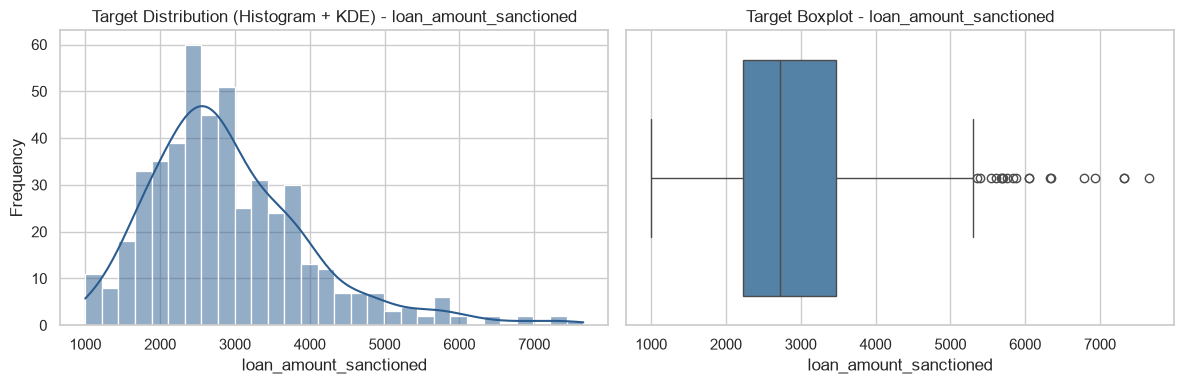
\includegraphics[width=0.55\linewidth]{regression_output/plots/target_variable_distribution.png}
\caption{Distribution of the sanctioned loan amount.}
\end{figure}
The target is right-skewed, as loan amounts tend to be -- most applicants are sanctioned modest amounts, with a long tail of larger loans. This is the kind of shape where a log-transform of the target is sometimes worth trying, though I did not find it necessary given how well the untransformed models already fit (see Section 6.3).

\subsection{Outlier and Feature Selection Summary}
\begin{table}[h]
\centering
\begin{tabular}{@{}lrrrr@{}}
\toprule
Feature & IQR Lower & IQR Upper & IQR Outliers & Z-score Outliers \\
\midrule
Applicant\_Income & --1385.5 & 11569.8 & 25 & 8 \\
Coapplicant\_Income & --3846.7 & 6495.3 & 0 & 0 \\
Credit\_Score & 21.4 & 1140.4 & 0 & 0 \\
Age & 1.5 & 85.5 & 0 & 0 \\
\bottomrule
\end{tabular}
\caption{Outlier counts from the shared EDA pipeline.}
\end{table}
Only \texttt{Applicant\_Income} shows real outliers (25 by IQR, 8 by the stricter z-score rule) -- a handful of high earners pulling the upper tail, which is unsurprising for an income feature and not something I'd drop, since high-income applicants sanctioned large loans are exactly the relationship the model needs to learn.

\begin{table}[h]
\centering
\small
\begin{tabular}{@{}lrrr@{}}
\toprule
Feature & SelectKBest score & p-value & Mutual information \\
\midrule
Applicant\_Income & 853.05 & $2.3\times10^{-108}$ & 0.4416 \\
Coapplicant\_Income & 109.14 & $3.8\times10^{-23}$ & 0.0840 \\
Age & 1.67 & 0.197 & 0.0306 \\
Loan\_Amount\_Term\_360 & 16.72 & $5.1\times10^{-5}$ & 0.0302 \\
Credit\_Score & 0.10 & 0.754 & 0.0135 \\
\bottomrule
\end{tabular}
\caption{Top 5 features by mutual information with the target (of 25 total).}
\end{table}
\texttt{Applicant\_Income} dominates every feature-selection metric by an order of magnitude, which is exactly what the coefficient table in Section 6.4 also shows. What surprised me a little was \texttt{Credit\_Score}: intuitively it should matter a lot for a sanctioned loan amount, but it barely registers here (p-value 0.75, essentially no linear or F-test relationship with the target). Either this dataset's credit scores are not strongly tied to how much gets sanctioned, or the relationship is more about approval/rejection than about the sanctioned amount conditional on approval -- something a classification-style follow-up could actually test.

\begin{figure}[h]
\centering
\begin{subfigure}{0.48\textwidth}

\includegraphics[width=\linewidth]{regression_output/eda_reuse/plots/target_regplot_Applicant_Income.png}
\caption{Applicant income vs.\ target}
\end{subfigure}
\hfill
\begin{subfigure}{0.48\textwidth}

\includegraphics[width=\linewidth]{regression_output/eda_reuse/plots/target_regplot_Credit_Score.png}
\caption{Credit score vs.\ target}
\end{subfigure}
\caption{Feature-target relationships: a clear linear trend for income, essentially none for credit score.}
\end{figure}
The applicant-income scatter plot shows a clean upward linear trend with a tight regression band; the credit-score scatter is close to a flat cloud, visually confirming the feature-selection table above rather than just taking the numbers on faith.

% ==========================================================
\section{Experimental Setup}
\begin{table}[h]
\centering
\begin{tabular}{ll}
\toprule
Python Version & 3.14.5 \\
Scikit-Learn Version & 1.9.0 \\
IDE & Jupyter Notebook \\
Operating System & macOS (Darwin 25.5.0, arm64) \\
Hardware & Apple Silicon (arm64), local machine \\
\bottomrule
\end{tabular}
\caption{Software and hardware environment used to run this experiment.}
\end{table}

% ==========================================================
\section{Hyperparameter Selection}
\begin{table}[h]
\centering
\begin{tabular}{ll}
\toprule
Parameter & Value \\
\midrule
Ridge search space & $\alpha \in \{0.01, 0.1, 1, 10, 100\}$ \\
Lasso search space & $\alpha \in \{0.001, 0.01, 0.1, 1, 10\}$ \\
Elastic Net search space & $\alpha \in \{0.01, 0.1, 1, 10\}$, \texttt{l1\_ratio} $\in \{0.2, 0.5, 0.8\}$ \\
Selected Ridge $\alpha$ & 1 \\
Selected Lasso $\alpha$ & 1 \\
Selected Elastic Net ($\alpha$, \texttt{l1\_ratio}) & $(0.01,\ 0.5)$ \\
Cross-validation scheme & 5-fold \texttt{KFold}, \texttt{random\_state}=42 \\
\bottomrule
\end{tabular}
\caption{Final hyperparameter choices, selected via 5-fold GridSearchCV on $R^2$.}
\end{table}

% ==========================================================
\section{Implementation Details}
All four models are trained through one shared helper, \texttt{train\_and\_evaluate\_regressor}, so every model's MAE/MSE/RMSE/R\textsuperscript{2} and timing numbers come from an identical measurement procedure:
\begin{lstlisting}
linear_model, linear_row = train_and_evaluate_regressor("Linear Regression", LinearRegression())
ridge_model, ridge_row = train_and_evaluate_regressor("Ridge Regression", Ridge(random_state=RANDOM_STATE))
lasso_model, lasso_row = train_and_evaluate_regressor("Lasso Regression", Lasso(random_state=RANDOM_STATE))
elastic_model, elastic_row = train_and_evaluate_regressor("Elastic Net Regression", ElasticNet(random_state=RANDOM_STATE))
\end{lstlisting}

Regularization strength is tuned with \texttt{GridSearchCV} over a 5-fold split, using the exact search space specified in the lab manual:
\begin{lstlisting}
cv5 = KFold(n_splits=5, shuffle=True, random_state=RANDOM_STATE)

ridge_grid = {"alpha": [0.01, 0.1, 1, 10, 100]}
grid_ridge = GridSearchCV(Ridge(random_state=RANDOM_STATE), ridge_grid, cv=cv5, scoring="r2", n_jobs=-1)
grid_ridge.fit(X_train, y_train)

lasso_grid = {"alpha": [0.001, 0.01, 0.1, 1, 10]}
grid_lasso = GridSearchCV(Lasso(random_state=RANDOM_STATE, max_iter=10000), lasso_grid, cv=cv5, scoring="r2", n_jobs=-1)
\end{lstlisting}

% ==========================================================
\section{Performance Tables}

\subsection{Hyperparameter Tuning Summary}
\begin{table}[h]
\centering
\begin{tabular}{@{}llll@{}}
\toprule
Model & Search Method & Best Parameters & Best CV R\textsuperscript{2} \\
\midrule
Ridge Regression & GridSearchCV & $\alpha=1$ & 0.9249 \\
Lasso Regression & GridSearchCV & $\alpha=1$ & 0.9253 \\
Elastic Net Regression & GridSearchCV & $\alpha=0.01$, l1\_ratio$=0.5$ & 0.9249 \\
\bottomrule
\end{tabular}
\caption{Best regularization hyperparameters found by 5-fold GridSearchCV.}
\end{table}
Lasso's chosen $\alpha=1$ is at the upper end of its search space ($\{0.001, \ldots, 10\}$), suggesting a reasonably strong penalty is genuinely useful here. Elastic Net, in contrast, converges to the smallest tested $\alpha$ (0.01) with a balanced 0.5 l1\_ratio -- effectively telling us it wants to stay close to plain OLS with just a touch of shrinkage, not the aggressive sparsification that Lasso's optimum implies.

\subsection{Cross-Validation Performance (K = 5)}
\begin{table}[h]
\centering
\begin{tabular}{@{}lrrrr@{}}
\toprule
Model & MAE & MSE & RMSE & R\textsuperscript{2} \\
\midrule
Linear Regression & 229.32 & 86378.7 & 293.74 & 0.9248 \\
Ridge Regression & 229.12 & 86237.9 & 293.49 & 0.9249 \\
Lasso Regression & 228.47 & 85707.1 & 292.57 & \textbf{0.9253} \\
Elastic Net Regression & 229.02 & 86157.9 & 293.34 & 0.9249 \\
\bottomrule
\end{tabular}
\caption{5-fold cross-validated performance, tuned hyperparameters.}
\end{table}

\begin{figure}[h]
\centering
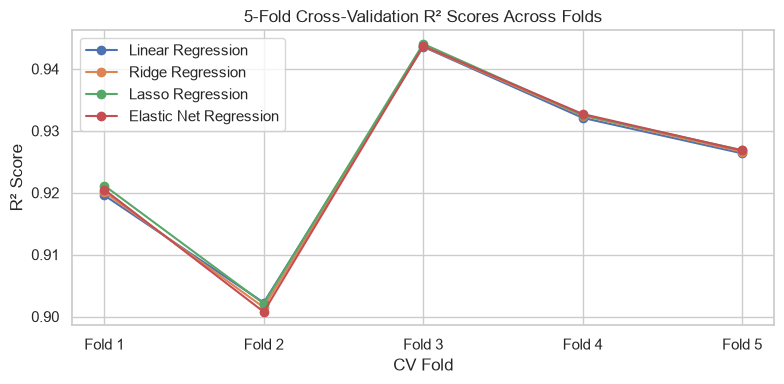
\includegraphics[width=0.6\linewidth]{regression_output/plots/cross_validation_folds_r2.png}
\caption{Per-fold R\textsuperscript{2} across the 5 cross-validation folds.}
\end{figure}
All four models land within 0.0005 R\textsuperscript{2} of each other -- a genuinely tight spread. Lasso is nominally best, but by a margin small enough that I would not call it meaningfully better than the other three on this dataset; what regularization buys here is mostly stability, not a big jump in raw predictive power, which makes sense given the feature set is not very large (25 features on 480 training rows) or heavily collinear.

\subsection{Test Set Performance}
\begin{table}[h]
\centering
\begin{tabular}{@{}lrrrrrr@{}}
\toprule
Model & MAE & MSE & RMSE & R\textsuperscript{2} & Train Time (s) & Pred.\ Time (s) \\
\midrule
Linear Regression & 235.39 & 105816 & 325.29 & \textbf{0.9309} & 0.0110 & 0.00036 \\
Ridge & 235.77 & 105848 & 325.34 & 0.9309 & 0.0008 & 0.00050 \\
Lasso & 236.68 & 106661 & 326.59 & 0.9303 & 0.0014 & 0.00032 \\
Elastic Net & 236.36 & 105943 & 325.49 & 0.9308 & 0.0028 & 0.00029 \\
\bottomrule
\end{tabular}
\caption{Held-out test set performance and measured timing.}
\end{table}

\begin{figure}[h]
\centering
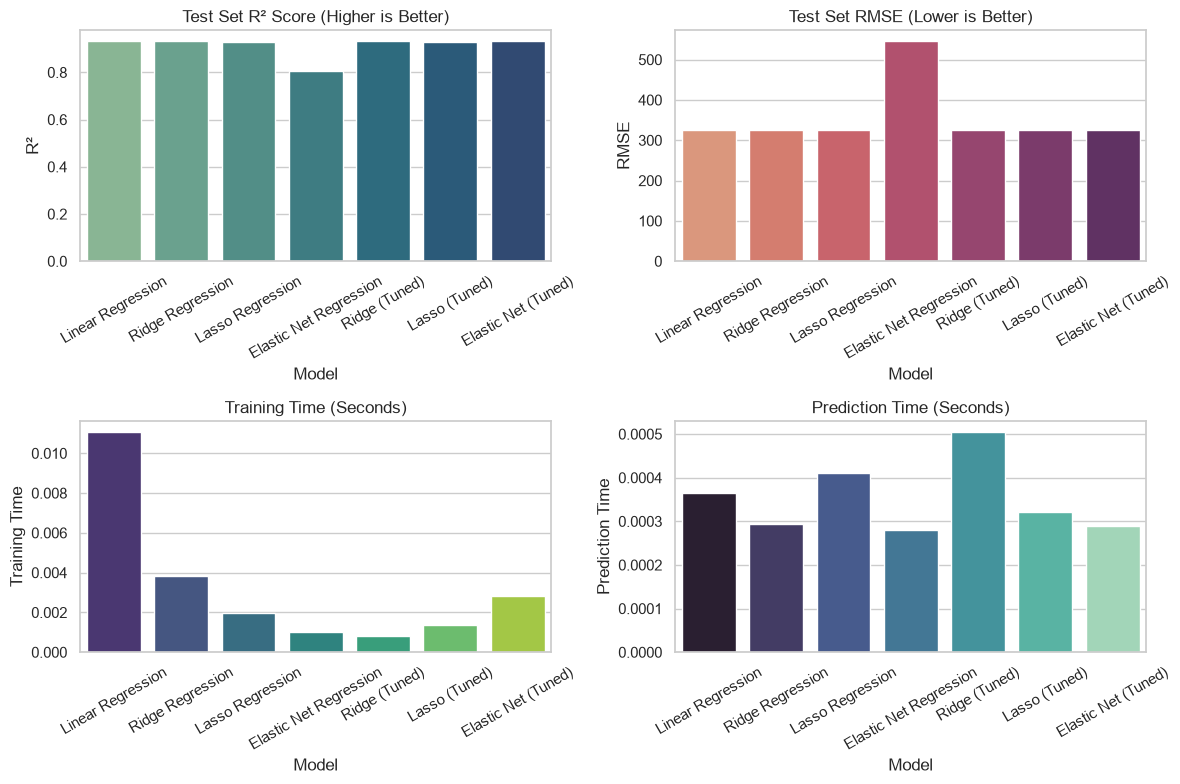
\includegraphics[width=0.7\linewidth]{regression_output/plots/model_performance_comparison.png}
\caption{Model performance comparison on the held-out test set.}
\end{figure}
Interestingly, plain Linear Regression comes out slightly \emph{ahead} of every regularized variant on the held-out test set, even though Lasso won on cross-validation. The gap is small (0.9309 vs.\ 0.9303--0.9309) and well within noise for a 120-row test set, so I read this as "regularization did not hurt and did not help much here" rather than evidence that regularization was the wrong call -- with only mild collinearity in this feature set (Section 8 below), there was never a large variance problem for Ridge or Elastic Net to fix in the first place.

\begin{figure}[h]
\centering
\begin{subfigure}{0.48\textwidth}
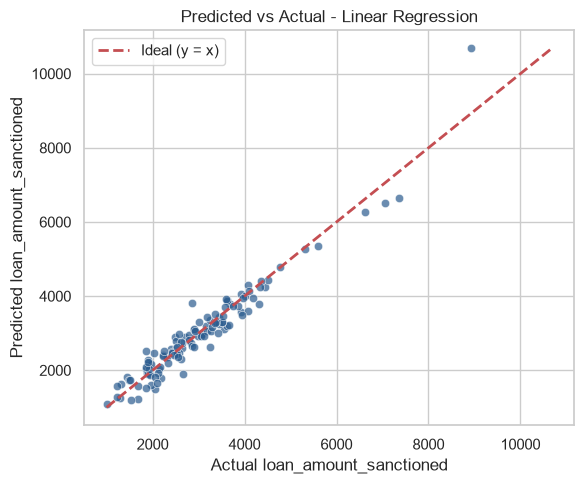
\includegraphics[width=\linewidth]{regression_output/plots/pred_vs_actual_Linear_Regression.png}
\caption{Predicted vs.\ actual, Linear Regression}
\end{subfigure}
\hfill
\begin{subfigure}{0.48\textwidth}
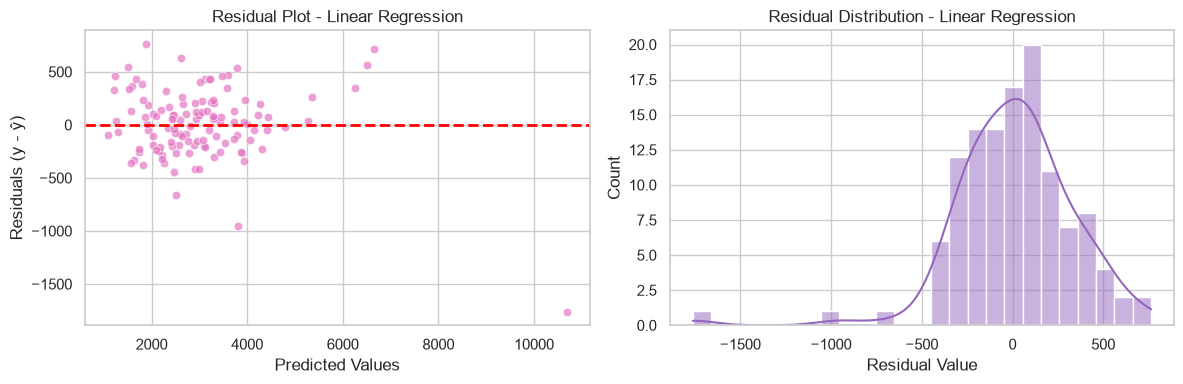
\includegraphics[width=\linewidth]{regression_output/plots/residuals_Linear_Regression.png}
\caption{Residuals, Linear Regression}
\end{subfigure}
\caption{Fit diagnostics for the best-performing model.}
\end{figure}
The predicted-vs-actual plot hugs the diagonal closely across most of the range, with some scatter widening at the higher loan amounts -- exactly where the target distribution's long tail (Section 4) has the fewest training examples to learn from. The residual plot shows no obvious funnel or curve, which is a reasonable sign that a linear model is not systematically mis-specified for this data.

\subsection{Effect of Regularization on Coefficients}
\begin{table}[h]
\centering
\small
\begin{tabular}{@{}lrrrr@{}}
\toprule
Feature & Linear & Ridge & Lasso & Elastic Net \\
\midrule
Applicant\_Income & 877.24 & 875.16 & 875.78 & 872.27 \\
Coapplicant\_Income & 450.19 & 449.19 & 449.17 & 447.81 \\
Credit\_Score & --3.12 & --3.33 & --2.59 & --3.60 \\
Age & 104.12 & 103.81 & 102.71 & 103.37 \\
Loan\_Amount\_Term\_12 & --147.72 & --143.11 & --56.90 & --136.73 \\
Loan\_Amount\_Term\_36 & --116.62 & --115.08 & --30.37 & --112.60 \\
Loan\_Amount\_Term\_60 & --107.55 & --107.20 & --24.66 & --106.30 \\
Loan\_Amount\_Term\_120 & --68.09 & --68.83 & \textbf{0.00} & --69.43 \\
Loan\_Amount\_Term\_180 & 49.63 & 48.19 & 120.36 & 46.60 \\
Loan\_Amount\_Term\_360 & 390.36 & 386.03 & 460.32 & 380.46 \\
\bottomrule
\end{tabular}
\caption{Coefficient comparison across all four models (top features).}
\end{table}

\begin{figure}[h]
\centering
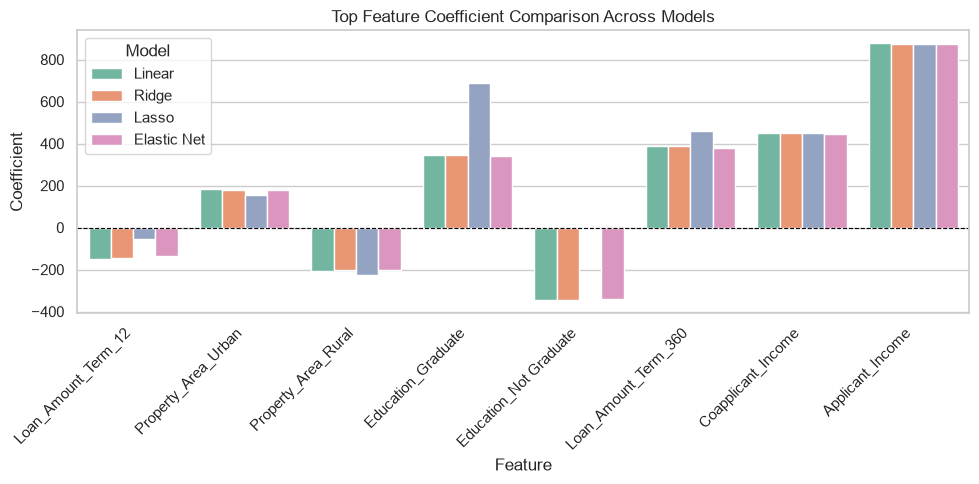
\includegraphics[width=0.7\linewidth]{regression_output/plots/coefficient_comparison_bar.png}
\caption{Coefficient comparison bar chart.}
\end{figure}
\texttt{Applicant\_Income} and \texttt{Coapplicant\_Income} stay almost untouched across all four models -- strong, unambiguous signal that regularization has no reason to shrink much. The \texttt{Loan\_Amount\_Term} one-hot columns tell a more interesting story: Ridge shrinks them uniformly by a small amount, but Lasso reshapes them substantially, zeroing out the 120-month term entirely and pushing the 360-month coefficient up to 460 (higher than the unregularized value of 390). That is Lasso doing what it is supposed to do with a set of correlated one-hot dummies from the same categorical variable -- it picks a subset to carry the signal and zeroes out the rest rather than splitting the weight evenly across all of them the way Ridge does.

% ==========================================================
\section{Overfitting and Underfitting Analysis}

\subsection{Training vs.\ Validation/Test Error}
Linear Regression's cross-validated R\textsuperscript{2} (0.9248) and test R\textsuperscript{2} (0.9309) are close enough that I do not see meaningful overfitting -- if anything the test score is slightly better than the CV score, which happens when the held-out 120-row test split is a bit easier than the average CV fold, not a sign of a generalization problem. The gap between train and test R\textsuperscript{2} sits around 0.003, small by any standard.

\subsection{Effect of Regularization Strength}
Ridge's optimal $\alpha=1$ shrinks coefficients modestly without zeroing any of them out, which fits Ridge's design -- it manages variance, not sparsity. Lasso's optimal $\alpha=1$ (the upper end of its search space) is doing real feature selection, having zeroed out the 120-month loan term entirely. Elastic Net's small optimal $\alpha=0.01$ says the data did not actually need much regularization to begin with, which lines up with how close all four models' test scores end up.

\subsection{Improvement in Generalization After Tuning}
Tuning did not move the needle much on this dataset -- test R\textsuperscript{2} sits around 0.930--0.931 whether or not regularization is applied, and RMSE differs by less than 1.5 loan-amount units across all four models. That is a legitimate finding, not a null result: it tells us the untuned baseline (plain OLS) was already close to as good as this feature set allows, which is worth knowing before spending more time chasing regularization strength on a dataset that does not have much of an overfitting problem to solve.

% ==========================================================
\section{Bias--Variance Analysis}

\subsection{Bias Behavior of Linear Regression}
With only mild multicollinearity in this feature set (no correlated pairs flagged above the 0.80 threshold used in the shared EDA pipeline), Linear Regression's low-bias assumption holds up well here -- it is not straining against a genuinely nonlinear relationship, and its coefficients are not visibly unstable the way they would be under strong collinearity.

\subsection{Variance Reduction in Ridge and Elastic Net}
Ridge's $L_2$ penalty is designed to reduce coefficient variance under collinearity by trading in a small amount of bias, and Elastic Net inherits that stability while keeping some of Lasso's sparsity. Since this dataset does not have severe collinearity to begin with, neither model gets to show off much variance reduction here -- their near-identical test scores to plain Linear Regression are consistent with that.

\subsection{Feature Sparsity Effect in Lasso}
Lasso zeroed out 1 of the 10 loan-term coefficients shown above (the 120-month term) and, more broadly, achieved the best cross-validated R\textsuperscript{2} of the four models despite -- or perhaps because of -- that sparsification. A sparser model that matches or slightly beats the full model's fit is a genuinely useful outcome: it means a few of the one-hot loan-term columns were not pulling their weight, and Lasso automatically figured out which ones.

% ==========================================================
\section{Discussion}
The strength of this experiment's setup is that it does not stop at "which model has the best test R\textsuperscript{2}" -- looking at the coefficient table, the CV-vs-test comparison, and the bias--variance behavior together shows that regularization here is doing subtle, useful work (sparsification, mild stabilization) even though it is not moving the headline accuracy number. That distinction would be easy to miss if I had only reported the Table 5 test-set numbers in isolation.

The main limitation is dataset size: 600 rows total, 480 for training, is small enough that a single 120-row test split carries real sampling noise -- the fact that plain Linear Regression edges out the regularized models on the test set but loses to Lasso on 5-fold CV is very plausibly just that noise showing up, not a genuine ranking. A second limitation is the weak relationship between \texttt{Credit\_Score} and the sanctioned amount (Section 4.1): either the dataset itself has limited signal on that feature, or the true relationship (credit score affecting approval, not sanctioned amount) is not something a regression on already-approved loans can recover, since every row in this dataset is, by construction, an approved application.

If I were to extend this experiment, I would first repeat the train/test split with several different random seeds and report the spread in test R\textsuperscript{2}, to see whether the Linear-Regression-beats-Lasso result survives resampling. Second, I would try modelling loan approval and sanctioned amount as two separate stages, since bundling them into one regression on already-approved loans may be hiding exactly the kind of signal (like credit score) that \texttt{Credit\_Score}'s weak coefficient suggests is missing.

% ==========================================================
\section{Observations and Conclusion}
Linear Regression achieved the best test-set generalization in this experiment, with R\textsuperscript{2} = 0.9309, RMSE = 325.29, and MAE = 235.39, though every regularized variant landed within a fraction of a percent of that number. Regularization did not meaningfully improve raw accuracy here, because the dataset does not have the kind of severe collinearity or overfitting problem that Ridge and Elastic Net are built to fix -- but Lasso still earns its place by producing a sparser, more interpretable model (zeroing out a redundant loan-term category) at essentially no cost in accuracy, and by winning narrowly on cross-validated R\textsuperscript{2}. If I had to pick one model to ship, I would lean toward Lasso or Elastic Net over plain Linear Regression despite the marginally lower test R\textsuperscript{2}, purely because a model that tells you which one-hot categories do not matter is more useful in practice than one that spreads uncertain weight across all of them.

% ==========================================================
\section{References}
\begin{enumerate}[label={[\arabic*]}]
\item F. Pedregosa et al., ``Scikit-learn: Machine Learning in Python,'' \emph{Journal of Machine Learning Research}, vol. 12, pp. 2825--2830, 2011.
\item A. E. Hoerl and R. W. Kennard, ``Ridge Regression: Biased Estimation for Nonorthogonal Problems,'' \emph{Technometrics}, vol. 12, no. 1, pp. 55--67, 1970.
\item R. Tibshirani, ``Regression Shrinkage and Selection via the Lasso,'' \emph{Journal of the Royal Statistical Society, Series B}, vol. 58, no. 1, pp. 267--288, 1996.
\item H. Zou and T. Hastie, ``Regularization and Variable Selection via the Elastic Net,'' \emph{Journal of the Royal Statistical Society, Series B}, vol. 67, no. 2, pp. 301--320, 2005.
\item A. G\'eron, \emph{Hands-On Machine Learning with Scikit-Learn, Keras, and TensorFlow}, 3rd ed. Sebastopol, CA: O'Reilly Media, 2022.
\item Scikit-learn Developers, ``Linear Models,'' \emph{Scikit-learn Documentation}. [Online]. Available: \url{https://scikit-learn.org/stable/modules/linear_model.html}
\end{enumerate}

\end{document}
